Seja $N$ um inteiro positivo. Uma coleção de $4N^2$ quadradinhos unitários com o desenho mostrado abaixo é organizada em um tabuleriro $2N\times2N$. Os quadradinhos podem ser rotacionados.
\begin{center}
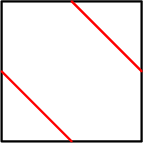
\includegraphics[width = 14.4mm]{img/fig0.png}
\end{center}
Os segmentos nos quadradinhos definem caminhos no tabuleiro. Determine o menor e o maior número possível de tais caminhos.

\textit{Por exemplo, existem $9$ caminhos no tabuleiro $4\times 4$ mostrado abaixo.}
\begin{center}
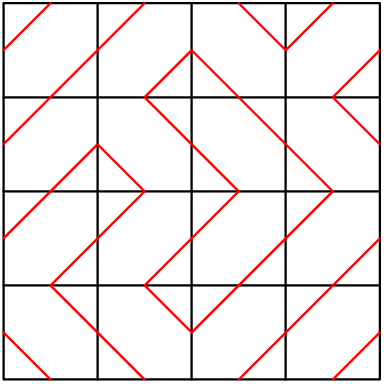
\includegraphics[width = 38.400000000000006mm]{img/fig1.png}
\end{center}
